%%%%%%%%%%%%%%%%%%%%%%%%%%%%%%%%%%%%

\section{2.5. Distribuições contínuas}

%%%%%%%%%%%%%%%%%%%%%%%%%%%%%%%%%%%%

\begin{frame}
\frametitle{Distribuições contínuas}

\begin{itemize}
\justifying
\item Abaixo um histograma da distribuição da altura de adultos. 
\justifying
\item A proporção de dados que cai nas caixas sombreadas dá a probabilidade de um adulto amostrado aleatoriamente ter entre 180cm e 185cm.

\end{itemize}

\begin{center}
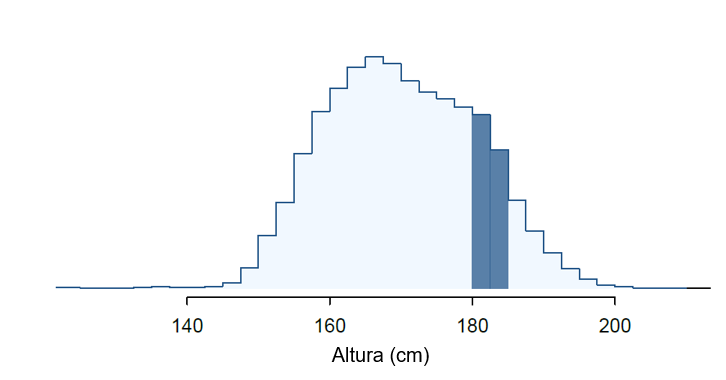
\includegraphics[width=0.75\textwidth]{2-5_continuous_distributions/usHeightsHist180185.png}
\end{center}


\end{frame}

%%%%%%%%%%%%%%%%%%%%%%%%%%%%%%%%%%%%

\subsection{Histogramas de distribuições contínuas}

\begin{frame}
\frametitle{Histogramas de distribuições contínuas}
\justifying
Como a altura é uma variável numérica contínua, sua \hl{função densidade de probabilidade} é uma curva suave.

\begin{center}
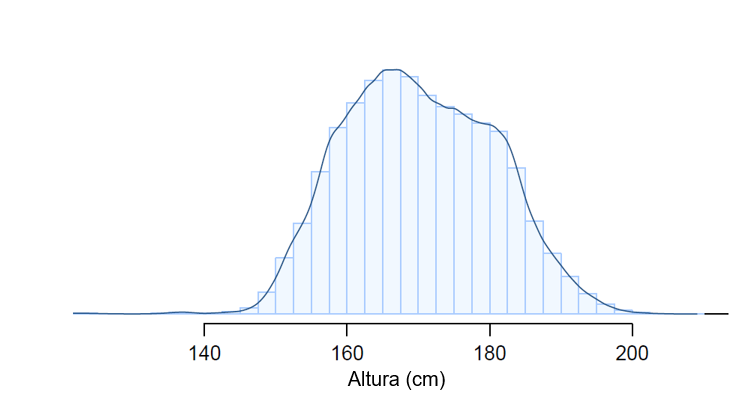
\includegraphics[width=\textwidth]{2-5_continuous_distributions/fdicHeightContDist.png}
\end{center}

\end{frame}

%%%%%%%%%%%%%%%%%%%%%%%%%%%%%%%%%%%%

\subsection{Distribuições contínuas}

\begin{frame}
\frametitle{Probabilidades de distribuições contínuas}
\justifying
A probabilidade de um adulto selecionado aleatoriamente ter entre 180cm e 185cm também pode ser estimada como a área sombreada sob a curva.

\begin{center}
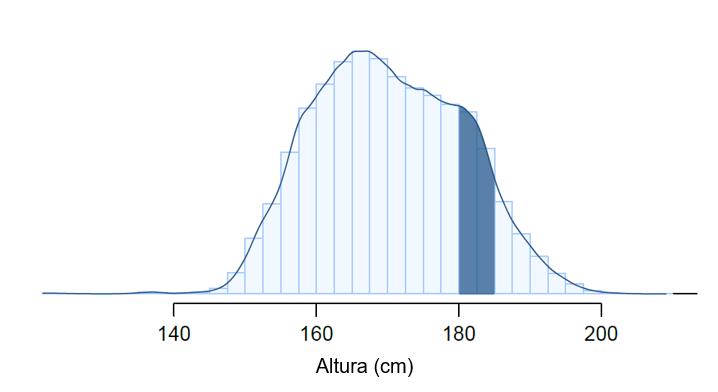
\includegraphics[width=\textwidth]{2-5_continuous_distributions/fdicHeightContDistFilled.png}
\end{center}


\end{frame}

%%%%%%%%%%%%%%%%%%%%%%%%%%%%%%%%%%%%

\begin{frame}
\frametitle{Por definição...}
\justifying
A probabilidade é estimada como "a área sob a curva", a probabilidade de uma pessoa ter exatamente 180cm (ou qualquer valor exato) é definida como 0.

\begin{center}
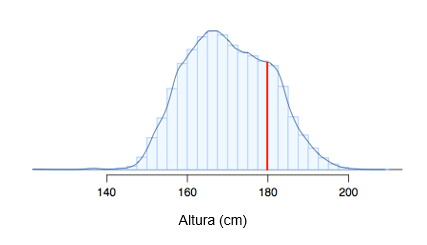
\includegraphics[width=0.8\textwidth]{2-5_continuous_distributions/fdicHeightContDist180.png}
\end{center}

\end{frame}

%%%%%%%%%%%%%%%%%%%%%%%%%%%%%%%%%%%%
